% Mirror: https://github.com/SIGma-UIUC/presentation-format
% --------------------------------------------------------------------
% This is a simple Beamer document that uses beamerthemesigma.sty
% Reading the comments should help you create a presentation even if
% you've never used Beamer before.
% --------------------------------------------------------------------

% Set our document class to Beamer
% \documentclass[aspectratio=169]{beamer}
\documentclass[aspectratio=169, handout]{beamer}
% Add handout option to ignore pauses

% From Jeff E
\usepackage{algo}
% Some more macros
\usepackage{sigmastyle}

\usepackage{tikz}
\usetikzlibrary{graphs}
\usetikzlibrary{arrows.meta}


% Set a title
\title{P vs NP: Complexity Classes with Graphs}

% Set a subtitle if you desire
\subtitle{Welcome Back!}

% Whoever worked on the presentation:
\author{SIGma}

% Date looks ugly, so leave blank
\date{}

% An institute name, if you're so inclined
% \institute{University of Illinois Urbana-Champaign}

% Use the SIGma theme for this Beamer presentation
\usetheme{sigma}
% --------------------------------------------------------------------

% Begin document
\begin{document}

% Beamer calls each slide a "frame", defined within the environment:
% \begin{frame}
%   <frame content here>
% \end{frame}

% This frame is just the title.
\begin{frame}
\titlepage
\end{frame}

% A frame with the table of contents.
% This frame's title is "Outline".
\begin{frame}{Outline}
  \tableofcontents
\end{frame}


\begin{frame}{Housekeeping}
    \centering
\includegraphics[width=0.25\textwidth]{qr-code.png}
    \begin{itemize}
        \item Join the Discord!
    \end{itemize}
\end{frame}


\section{Admins in No Particular Order}
\frame{\sectionpage}

\begin{frame}{Sasha}
    \begin{itemize}
        \item Sophomore in CS, double major in physics
        \item CA for CS 374
        \item Working on quantum cryptography research
        \item Participated in error-correcting codes research at USF REU this summer
    \end{itemize}
\end{frame}


\begin{frame}{Alex}
    \begin{itemize}
        \item Junior in Stats \& CS, double major in Math
        \item CA for CS 225, previously a CA for CS 128H and CS 374
        \item Doing compilers adjacent research
        \item SWE intern at Box this summer
    \end{itemize}
\end{frame}


\begin{frame}{Franklin}
    \begin{itemize}
        \item Junior in Math \& CS
        \item CA for CS 374
        \item SWE internship at CME Group this summer
    \end{itemize}
\end{frame}


\begin{frame}{Ryan}
    \begin{itemize}
        \item 
    \end{itemize}
\end{frame}


\begin{frame}{Sam}
    \begin{itemize}
        \item CS PhD, in TCS, 2nd year
        \item VR/RE Intern @ Battelle
        \item SIGma Admin since Fall 2022
    \end{itemize}
\end{frame}


\begin{frame}{Porter}
    \begin{itemize}
        \item CS Major; Math Minor; 2 years left in B.S.-M.C.S.
        \item SWE internship at CDK Global this summer
        \item CA for CS 128H and CS 225
        \item Second semester as a SIGma Admin
        \item Cardio King and Foosball Fanatic
    \end{itemize}
\end{frame}



\section{Graphs}
\frame{\sectionpage}


\begin{frame}{Definitions}
    \begin{itemize}
        \item In computer science and abstract math, graphs are a very specific thing. \pause
        \item A graph, \emph{G}, consists of a set of vertices, \emph{V}, and a set of edges, \emph{E}.\pause
        \begin{itemize}
            \item $G = (V, E)$
        \end{itemize}
    \end{itemize}
    \begin{center}
        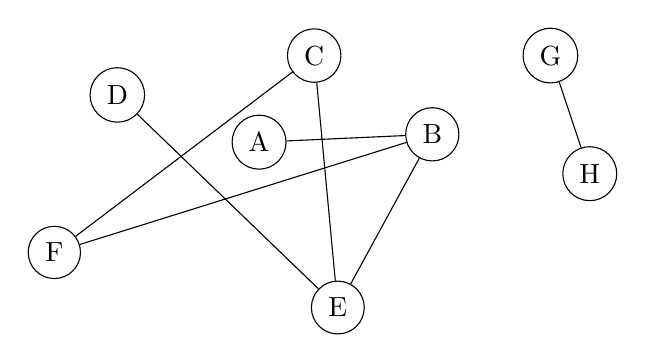
\begin{tikzpicture} [every node/.style={draw,circle}]
            \node (a) at (0.3, -0.1)    {A};
            \node (b) at (2.5, 0)       {B};
            \node (c) at (1, 1)         {C};
            \node (d) at (-1.5, 0.5)    {D};
            \node (e) at (1.3, -2.2)    {E};
            \node (f) at (-2.3, -1.5)   {F};
            \node (g) at (4, 1)         {G};
            \node (h) at (4.5, -0.5)    {H};

            \graph[edges={-}] {
                (a) -- (b) -- (e) -- (c);
                (b) -- (f) -- (c);
                (d) -- (e);
                (g) -- (h);
            };
        \end{tikzpicture}
    \end{center}
\end{frame}

\begin{frame}{Definitions}
    Graphs can be directed...
    \begin{center}
        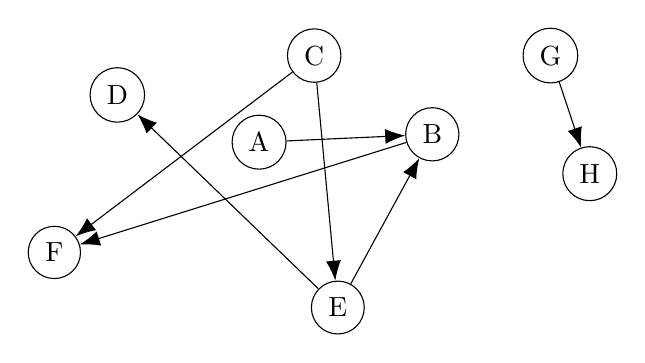
\begin{tikzpicture} [every node/.style={draw,circle}]
            \node (a) at (0.3, -0.1)    {A};
            \node (b) at (2.5, 0)         {B};
            \node (c) at (1, 1)         {C};
            \node (d) at (-1.5, 0.5)    {D};
            \node (e) at (1.3, -2.2)    {E};
            \node (f) at (-2.3, -1.5)   {F};
            \node (g) at (4, 1)         {G};
            \node (h) at (4.5, -0.5)    {H};

            \begin{scope}[->, >={Latex[scale=1.5]}]
                \draw (a) -> (b);
                \draw (e) -> (b);
                \draw (c) -> (e);
                \draw (b) -> (f);
                \draw (c) -> (f);
                \draw (e) -> (d);
                \draw (g) -> (h);
            \end{scope}
        \end{tikzpicture}
    \end{center}
\end{frame}


\begin{frame}{Definitions}
    ...or weighted.
    \begin{center}
        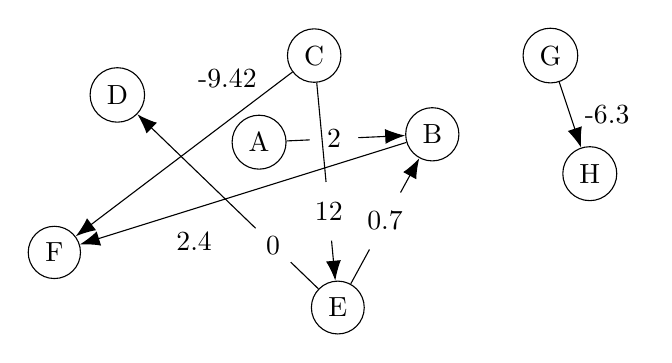
\begin{tikzpicture} [every node/.style={draw,circle}]
            \node (a) at (0.3, -0.1)    {A};
            \node (b) at (2.5, 0)       {B};
            \node (c) at (1, 1)         {C};
            \node (d) at (-1.5, 0.5)    {D};
            \node (e) at (1.3, -2.2)    {E};
            \node (f) at (-2.3, -1.5)   {F};
            \node (g) at (4, 1)         {G};
            \node (h) at (4.5, -0.5)    {H};

            \begin{scope}[->, >={Latex[scale=1.5]}]
                \draw (a) -> (b) node [pos=0.4, fill=white, draw=none] {2};
                \draw (e) -> (b) node [midway, fill=white, draw=none] {0.7};
                \draw (c) -> (e) node [pos=0.65, fill=white, draw=none] {12};
                \draw (b) -> (f) node [pos=0.65, below, draw=none] {2.4};
                \draw (e) -> (d) node [near start, fill=white, draw=none] {0};
                \draw (c) -> (f) node [pos=0.3, above, draw=none] {-9.42};
                \draw (g) -> (h) node [midway, right, draw=none] {-6.3};
            \end{scope}
        \end{tikzpicture}
    \end{center}
\end{frame}


\begin{frame}{Definitions Cont.}
    \begin{itemize}
        \item If one vertex can be reached by another, they are in the same \emph{connected component}. \pause
        \item The \emph{degree} of vertex $v$ is the number of edges with $v$ as an endpoint. \pause
        \item In a \emph{complete} graph, each vertex is connected to all other vertices with an edge. \pause
        \item \emph{Cycle}: what you get when it's possible to walk in a loop back to the starting vertex.
    \end{itemize}
\end{frame}


\begin{frame}{Maps}
    \begin{figure}
        \centering
        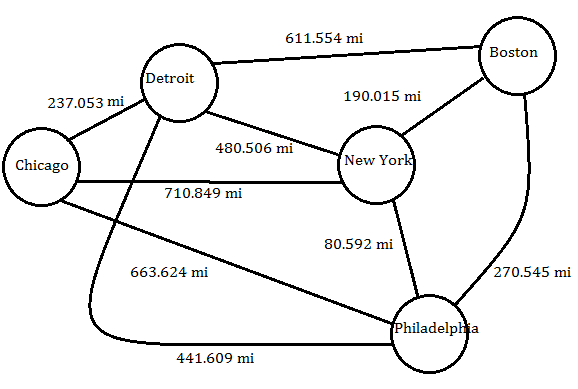
\includegraphics[width=0.75\linewidth]{map_graph.png}
    \end{figure}
\end{frame}


\begin{frame}{}
      \begin{center}
    {\color{sigma@mainblue} \LARGE Questions?}
  \end{center}
\end{frame}


\section{P vs NP}
\frame{\sectionpage}

\begin{frame}{Millennium Prize}
    \begin{itemize}
        \item On May 24, 2000, The Clay Mathematics Institute put a \$1 million reward on 7 unsolved "Millennium Problems". \pause
        \begin{itemize}
            \item Only one has been solved, but the winner, Grigori Perelman, turned down the prize due to "disagreement with the organized mathematical community."
        \end{itemize} \pause
        \item The question of P vs NP is one of the 6 remaining unsolved problems, and proof that $P = NP$ would have major implications in computing and beyond. \pause
        \begin{itemize}
            \item Cryptography
            \item Problem solving
        \end{itemize}
    \end{itemize}
\end{frame}


\begin{frame}{Background}
    \begin{itemize}
        \item Big-O analysis is used to analyze the runtime of an algorithm without getting bogged down by relatively insignificant details. \pause
        \begin{itemize}
            \item If an algorithm is \emph{$O(n)$}, runtime grows linearly to the size of the input. \pause
            \item For \emph{$O(n!)$} algorithms, runtime grows factorially to the size of the input. \pause
            \item $O(n) = O(\frac{n}{2}) = O(2000 \cdot n + 37) = O(c \cdot n)$ \pause
        \end{itemize}
        \item This type of thinking works because computers operate at scale. \pause
        \item A \emph{polynomial-time} algorithm has a runtime of the form $O(n^k)$ for some $k$. Notably, this excludes exponentials and factorials. \pause
        \item \emph{Deterministic}: a process with a predictable result for a given start state.
    \end{itemize}
\end{frame}


\begin{frame}{P vs NP}
    \begin{itemize}
        \item \emph{P}: the set of \textbf{decision} problems that a \textbf{deterministic} algorithm can solve in polynomial time. \pause
        \item \emph{NP}: the set of \textbf{decision} problems that a \textbf{nondeterministic} algorithm can solve in polynomial time. These problems can be \textbf{verifed} in polynomial time. \pause
        \item The big question: "Are these two types of problems truly different?" \pause
        \item Intuitively (and informally), this asks if problems that can be checked easily can also be solved easily. \pause
        \begin{itemize}
            \item (Intuitively, it feels like the answer should be no...)
        \end{itemize}
    \end{itemize}
\end{frame}

\begin{frame}{Example: Hamiltonian Cycle}
    \begin{itemize}
        \item Given a graph, does a cycle exist that visits each vertex exactly once?
    \end{itemize}
    \begin{center}
        \begin{tikzpicture} [every node/.style={draw,circle, minimum size=2em, color=sigma@mainblue}]
            \node (a) at (0.3, -0.1)    {E};
            \node (b) at (2.5, 0)       {D};
            \node (c) at (1, 1)         {H};
            \node (d) at (-1.5, 0.5)    {A};
            \node (e) at (1.3, -2.2)    {B};
            \node (f) at (-2.3, -1.5)   {I};
            \node (g) at (4, 1)         {G};
            \node (h) at (4.5, -2.5)    {F};
            \node (i) at (6, -0.5)      {C};

            \graph[edges={-}] {
                (f) -- (b) -- (e) -- (c);
            };
            \graph[edges={->, color=sigma@mainblue}] {
                (f) -- (d) -- (e) -- (i) -- (b) -- (a) -- (h) -- (g) -- (c) -- (f);
            };
        \end{tikzpicture}
    \end{center} \pause
    \begin{itemize}
        \item This is clearly verifiable in polynomial time. \pause
        \item A brute force algorithm is to try every possible path, which is $O(|V|!)$.
    \end{itemize}
\end{frame}


\begin{frame}{Hamilton's Clairvoyance}
    \begin{itemize}
        \item A nondeterministic algorithm is faster: imagine if we could correctly chose the right path at every junction. At that point, are we really solving anything? \pause
        \item By now, it should seem obvious that $P \ne NP$, but that has \textbf{not} been proven...
        \begin{itemize}
            \item ...so magic algorithms might be possible?! \pause
        \end{itemize}
        \item This particular problem is \emph{NP-complete}, which means every other problem in NP \emph{reduces} to it. 
    \end{itemize}
\end{frame}


\begin{frame}{}
      \begin{center}
    {\color{sigma@mainblue} \LARGE Questions?}
  \end{center}
\end{frame}


\section{Reductions and the Traveling Salesman}
\frame{\sectionpage}

\begin{frame}{But What Are Reductions?}
    We can show that a problem is in NP if we can use it to solve some other problem that we already know is in NP. This is a proof-by-contradiction of sorts.
\end{frame}

\begin{frame}{Traveling Salesman}
    Consider a salesman trying to visit some collection of cities on business before returning home. We ask: "Is it possible to visit these cities by traveling $\le k$ miles?"
    \\\\\\\\\\
    Is this problem NP-Hard?
\end{frame}

\begin{frame}{Traveling Salesman Reduction}
    \begin{itemize}
        \item Assume we have a polynomial-time algorithm to solve the TSP. \pause
        \item Now consider an instance of the Hamiltonian Cycle problem with graph $G = (V, E)$. \pause
        \item We want to use our TSP algorithm to find a Hamiltonian cycle. \pause
        \item Construct a new weighted graph, $G' = G$ with weights given by $w(u) = 1$ for $u \in V$. \pause
        \item Now we only have to run the TSP algorithm asking if it is possible to visit all the cities in $\le |V|$ miles. $G$ has a Hamiltonian Cycle if and only if the algorithm returns "yes."
    \end{itemize}
\end{frame}

\begin{frame}{Traveling Salesman Reduction Cont.}
    \begin{itemize}
        \item It took polynomial time to construct $G'$ from $G$, and our imagined TSP algorithm is also polynomial time, so the whole process took polynomial time. \pause
        \item But we believe the Hamiltonian Cycle problem is not solvable in polynomial time—a contradiction. \pause
        \item Thus, our initial assumption that a polynomial-time algorithm to solve the TSP exists is wrong, and the TSP is NP-hard.
    \end{itemize}
\end{frame}

\begin{frame}{}
      \begin{center}
    {\color{sigma@mainblue} \LARGE Questions?}
  \end{center}
\end{frame}

\begin{frame}{Current State of P vs NP}
    \begin{itemize}
        \item Most experts believe $P \ne NP$, but there is still no proof. \pause
        \item Many believe that we do not have the mathematical tools for a proof, or even that a proof is impossible in the common axiomatic systems that we have now. \cite{aaronson}
    \end{itemize}
\end{frame}


\section{Approximate Traveling Salesman}
\frame{\sectionpage}


\begin{frame}{Weekly Brainteaser}
    After the revolution, each of the 66 citizens of a certain city, including the king, has a salary of 1. King cannot vote, but has the power to suggest changes to the distribution of salaries. Each person's salary must be a \textbf{non-negative whole number of dollars}, and the salaries must sum to 66. He suggests a new salary plan for every person including himself in front of the city. Citizens are greedy, and vote yes if their salary is raised, no if decreased, and don't vote otherwise. The majority vote wins. The king proposes a series of plans to maximize his salary. \textbf{What is the king's maximum salary?}
\end{frame}



\begin{frame}[allowframebreaks]{Bibliography}
    \tiny
    \bibliography{refs}
    \bibliographystyle{alpha}
\end{frame}


\end{document}